\documentclass[11pt,a4paper]{article}
\usepackage[T1]{fontenc}
\usepackage[utf8]{inputenc}
\usepackage[a4paper,margin=2.5cm]{geometry}
\usepackage{amsmath}
\usepackage{graphicx}
\usepackage{booktabs}
\usepackage{caption}
\usepackage{tikz}
\usetikzlibrary{positioning,arrows.meta,fit,backgrounds,calc,shapes.geometric}
\usepackage[hidelinks]{hyperref}

\captionsetup{font=small}
\setlength{\parindent}{0pt}
\setlength{\parskip}{0.4em}
\renewcommand{\topfraction}{0.9}
\renewcommand{\bottomfraction}{0.8}
\renewcommand{\textfraction}{0.07}
\renewcommand{\floatpagefraction}{0.8}
\setlength{\textfloatsep}{10pt plus 2pt minus 2pt}

% Shared figure styles
\tikzset{
  box/.style={draw, rounded corners=2pt, align=center, font=\small, inner sep=4pt, fill=white},
  comp/.style={box, minimum width=3.4cm, minimum height=1.1cm, fill=blue!6},
  dev/.style={box, fill=gray!10, font=\footnotesize},
  soft/.style={box, fill=green!6, font=\footnotesize},
  dec/.style={draw, diamond, aspect=2.4, align=center, font=\footnotesize, inner sep=1pt, fill=orange!8},
  arr/.style={-{Stealth[length=2mm]}, thick},
  darr/.style={{Stealth[length=2mm]}-{Stealth[length=2mm]}, thick},
  lbl/.style={font=\scriptsize, align=center},
  group/.style={draw, dashed, rounded corners=4pt, inner sep=6pt},
}

\begin{document}
\begin{center}
  {\LARGE\bfseries Software Stack of the Lite3 Quadruped}\\[0.4em]
  {\large An overview of the control, perception, navigation and operator software}\\[0.8em]
  Håvard Karlsen Solheim, University of Agder, 2026
\end{center}
\begin{abstract}
\noindent This report presents the software stack that was implemented for a DEEP Robotics Lite3 Pro
quadruped, with the aim of letting the robot walk autonomously around a university campus while being
supervised from a desk. The stack was distributed over three on-board computers: the vendor's motion
computer, a perception computer running the Robot Operating System 2 (ROS~2) and the robot's
programming interface, and an added Orin Nano running the lidar, lidar-inertial odometry, map
localization, navigation and speech. At its core was the \texttt{Lite3} Python class, which turned the
robot's silent failure modes into automatic fixes or explicit errors and ended every motion with a stop
command. In tests, the robot reached all of its navigation goals in the lab, the surrounding hall and
across a bridge to the campus arcade, with a person carrying the handheld remote nearby.
\end{abstract}

\section{Introduction}

The Lite3 Pro is a commercial quadruped sold for research and education~\cite{deeprobotics}. Out of the
box it can be walked with a handheld remote, and it exposes a low-level network interface and a set of
ROS~2~\cite{ros2} nodes. The vendor controller also ignored commands without reporting why: in the wrong mode, lying
down, low on battery or not yet ``armed'', a velocity command simply had no effect. The software was
therefore built around two principles. Every silent failure was turned into an automatic fix or a clear
error, and whenever a program ended, normally, by an exception or by Ctrl-C, the last command it sent
to the legs was to stand still. These are
software measures; the handheld remote remained the robot's only hardware stop.

The research question was: \emph{How can an off-the-shelf quadruped be given a software stack that lets
it navigate a building autonomously, safely and under remote supervision?}

The work was carried out in the MAS518 Advanced Mechatronics Project, whose project description served
as a guideline. Of its four parts, this report covers robot configuration and teleoperation,
multi-sensor instrumentation and fusion (depth camera, lidar, inertial measurement unit (IMU) and
ultrasonic sensors), and simultaneous localization and mapping (SLAM) with autonomous navigation.
Kinematic modelling, reinforcement learning, simulation and the remaining sensors are left to a master thesis
(Section~\ref{sec:further}).

\section{Background}

Commercial quadrupeds such as ANYmal~\cite{anymal} split a real-time locomotion controller from a
separate computer for perception and autonomy, and research stacks for the Unitree Go2 follow the same
pattern~\cite{cmu}. Lidar-inertial odometry such as
FAST-LIO2 (Fast Lidar-Inertial Odometry)~\cite{fastlio2} estimates motion from a lidar and an IMU.
Localization on a prior map is often done by scan-to-map registration such as iterative closest point
(ICP)~\cite{icp}. Navigation in ROS~2 is commonly built on Nav2~\cite{nav2}: the Regulated Pure Pursuit
(RPP) controller~\cite{rpp} follows a path geometrically, while Model Predictive Path Integral (MPPI)
control~\cite{mppi} samples many candidate trajectories and follows the lowest-cost one. Odometry sources
are usually combined with an extended Kalman filter such as \texttt{robot\_localization}~\cite{robotloc}.
Such a filter rejects single outliers, but a lidar odometry that diverges gradually still pulls the
estimate away, which motivated the step-by-step gate used here (Section~\ref{sec:odom}).

\section{System Overview}

The robot used a ``split brain'' architecture, extended with a third computer on an Ethernet switch, as
shown in Figure~\ref{fig:hardware}.

\begin{figure}[htbp]
\centering
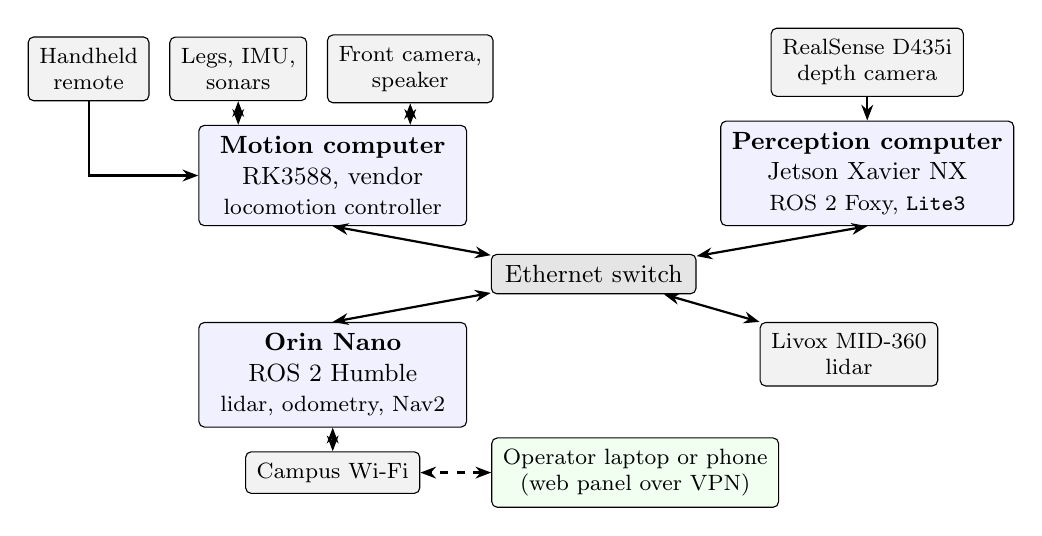
\begin{tikzpicture}[node distance=0.45cm and 0.6cm]
  \node[box, fill=gray!20, minimum width=2.6cm] (sw) {Ethernet switch};
  \node[comp, above left=0.35cm and 0.3cm of sw] (mot) {\textbf{Motion computer}\\ RK3588, vendor\\ \footnotesize locomotion controller};
  \node[comp, above right=0.35cm and 0.3cm of sw] (per) {\textbf{Perception computer}\\ Jetson Xavier NX\\ \footnotesize ROS 2 Foxy, \texttt{Lite3}};
  \node[comp, below left=0.35cm and 0.3cm of sw] (orin) {\textbf{Orin Nano}\\ ROS 2 Humble\\ \footnotesize lidar, odometry, Nav2};
  \node[dev, below right=0.35cm and 0.8cm of sw] (lidar) {Livox MID-360\\ lidar};
  \draw[darr] (mot.south) -- (sw);
  \draw[darr] (per.south) -- (sw);
  \draw[darr] (orin.north) -- (sw);
  \draw[darr] (lidar.north west) -- (sw);

  \node[dev, above=0.3cm of mot, xshift=-1.2cm] (legs) {Legs, IMU,\\ sonars};
  \node[dev, right=0.25cm of legs] (cam) {Front camera,\\ speaker};
  \node[dev, left=0.25cm of legs] (hand) {Handheld\\ remote};
  \draw[darr] (legs.south) -- (legs.south |- mot.north);
  \draw[darr] (cam.south) -- (cam.south |- mot.north);
  \draw[arr] (hand.south) |- (mot.west);

  \node[dev, above=0.3cm of per] (rs) {RealSense D435i\\ depth camera};
  \draw[arr] (rs) -- (per);

  \node[dev, below=0.3cm of orin] (wifi) {Campus Wi-Fi};
  \draw[darr] (wifi) -- (orin);
  \node[soft, right=0.9cm of wifi] (op) {Operator laptop or phone\\ (web panel over VPN)};
  \draw[darr, dashed] (op) -- (wifi);
\end{tikzpicture}
\caption{The robot's computers, sensors and network. The Orin also provided internet access to the
other computers over the campus Wi-Fi.}
\label{fig:hardware}
\end{figure}

The \emph{motion computer} ran the vendor's closed locomotion controller with its 1~kHz joint loop, and
carried the front camera, loudspeaker, ultrasonic sensors and the handheld's Wi-Fi access point. It was
treated as a black box that accepted commands over the User Datagram Protocol (UDP). The \emph{perception
computer} ran ROS~2 Foxy, the RealSense D435i depth camera~\cite{realsense}, the vendor's bridge to the
motion computer, the \texttt{Lite3} interface and the web panel. Being close to fully loaded, it was
relieved by the \emph{Orin Nano}, added with a Livox MID-360 lidar~\cite{livox}, which ran the lidar,
FAST-LIO2, map localization, the Nav2 controller and speech synthesis. The Orin was also the robot's
internet connection over the campus Wi-Fi. Remote access went through a Tailscale virtual private network (VPN), and the panel's video
streams ran only while a logged-in page displayed them; video was not stored, and a sign on the robot
told people about the cameras. As the Orin ran a newer ROS~2 with a different
middleware, the two computers exchanged data as small UDP datagrams through relay processes.

\section{The Lite3 Class}

All programs that commanded the robot were built on one Python class, \texttt{Lite3}, shown in
Figure~\ref{fig:lite3}. It was assembled from mixins sharing one ROS~2 node: the core handled state,
posture and motion, \texttt{Nav} added navigation, and \texttt{Depth} added obstacle ranges.

\begin{figure}[htbp]
\centering
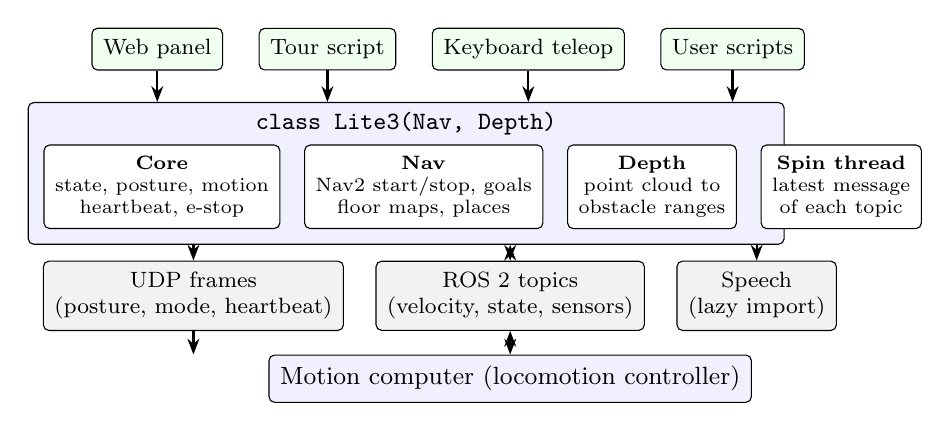
\begin{tikzpicture}[node distance=0.3cm and 0.45cm]
  \node[soft] (hmi) {Web panel};
  \node[soft, right=of hmi] (tour) {Tour script};
  \node[soft, right=of tour] (tele) {Keyboard teleop};
  \node[soft, right=of tele] (scr) {User scripts};

  \node[box, fill=blue!6, below=0.4cm of tour, xshift=1.0cm, minimum width=9.6cm, minimum height=1.8cm] (cls) {};
  \node[font=\small\bfseries, anchor=north] at (cls.north) {\texttt{class Lite3(Nav, Depth)}};
  \node[box, font=\scriptsize, anchor=south west] (core) at ([xshift=2mm, yshift=2mm]cls.south west)
       {\textbf{Core}\\ state, posture, motion\\ heartbeat, e-stop};
  \node[box, font=\scriptsize, right=0.3cm of core] (nav) {\textbf{Nav}\\ Nav2 start/stop, goals\\ floor maps, places};
  \node[box, font=\scriptsize, right=0.3cm of nav] (dep) {\textbf{Depth}\\ point cloud to\\ obstacle ranges};
  \node[box, font=\scriptsize, right=0.3cm of dep] (spin) {\textbf{Spin thread}\\ latest message\\ of each topic};
  \foreach \n in {hmi,tour,tele,scr} \draw[arr] (\n.south) -- (\n.south |- cls.north);

  \node[dev, below=0.4cm of core, xshift=0.4cm] (udp) {UDP frames\\ (posture, mode, heartbeat)};
  \node[dev, right=0.4cm of udp] (ros) {ROS 2 topics\\ (velocity, state, sensors)};
  \node[dev, right=0.4cm of ros] (tts) {Speech\\ (lazy import)};
  \draw[arr] (udp.north |- cls.south) -- (udp.north);
  \draw[darr] (ros.north |- cls.south) -- (ros.north);
  \draw[arr] (tts.north |- cls.south) -- (tts.north);
  \node[comp, below=0.3cm of ros, minimum height=0.6cm] (jy) {Motion computer (locomotion controller)};
  \draw[arr] (udp.south) -- (udp.south |- jy.north);
  \draw[darr] (ros.south) -- (jy.north);
\end{tikzpicture}
\caption{Structure of the \texttt{Lite3} class and the programs built on it. Commands reached the motion
computer as raw UDP frames or as ROS~2 velocity messages through the vendor bridge.}
\label{fig:lite3}
\end{figure}

On creation, the object selected the correct ROS~2 middleware, started a background thread that kept the
latest message of each topic, installed a Ctrl-C handler that triggered an emergency stop, and put the
robot into automatic mode. The robot's state was therefore available as plain attributes such as
\texttt{bot.battery} and \texttt{bot.pose}, and programs read as sequential Python without callbacks.
Posture, mode, heartbeat and tricks were sent as 12-byte UDP frames to the locomotion controller;
velocities went through \texttt{/cmd\_vel} and the vendor bridge.

\subsection{Posture and arming}

The controller reported a \emph{basic state}: not armed after power-on, arming, lying, in transition, or
standing, the only state that accepted velocities. It ignored all network commands unless a heartbeat
arrived at least twice per second; \texttt{heartbeat\_start()} let the program send it instead of the
handheld. Even then, the first command after power-on was swallowed by arming. Since the stand command
was a toggle, \texttt{stand()} and \texttt{sit()} were made idempotent: they returned at once if already in
the requested posture, refused to act from a transition, confirmed the result from the basic state, and
re-sent the toggle if the robot was still lying after 2~s.

\subsection{Motion and stopping}

All motion calls (\texttt{walk}, \texttt{turn}, \texttt{strafe}, \texttt{steer}) ran through one loop,
shown in Figure~\ref{fig:loop}. It published a velocity every 50~ms until the target was reached, a check
failed or 30~s passed, and ended in a \texttt{finally} block that published zero velocities, also after an
exception or Ctrl-C. Each call returned how far the robot had moved and why it stopped, for example
\texttt{'obstacle at 0.58 m'}, since stopping short is normal. Before a turn, the robot's footprint was
swept through the turn over Nav2's local costmap.

\begin{figure}[htbp]
\centering
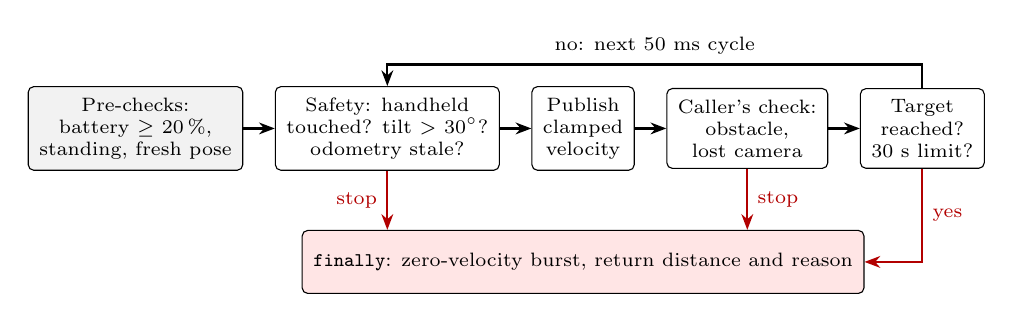
\begin{tikzpicture}[node distance=0.4cm, b/.style={box, font=\scriptsize, minimum height=1.0cm}]
  \node[b, fill=gray!10] (pre) {Pre-checks:\\ battery $\geq$ 20\,\%,\\ standing, fresh pose};
  \node[b, right=of pre] (safe) {Safety: handheld\\ touched? tilt $>$ 30$^\circ$?\\ odometry stale?};
  \node[b, right=of safe] (pub) {Publish\\ clamped\\ velocity};
  \node[b, right=of pub] (abort) {Caller's check:\\ obstacle,\\ lost camera};
  \node[b, right=of abort] (done) {Target\\ reached?\\ 30 s limit?};
  \node[b, fill=red!10, below=0.75cm of pub, minimum width=6cm, minimum height=0.8cm] (halt)
       {\texttt{finally}: zero-velocity burst, return distance and reason};
  \draw[arr] (pre) -- (safe);
  \draw[arr] (safe) -- (pub);
  \draw[arr] (pub) -- (abort);
  \draw[arr] (abort) -- (done);
  \draw[arr] (done.north) -- ++(0,0.3) -| node[lbl, pos=0.25, above] {no: next 50 ms cycle} (safe.north);
  \draw[arr, red!70!black] (safe.south) -- node[lbl, left] {stop} (safe.south |- halt.north);
  \draw[arr, red!70!black] (abort.south) -- node[lbl, right] {stop} (abort.south |- halt.north);
  \draw[arr, red!70!black] (done.south) |- node[lbl, pos=0.25, right] {yes} (halt.east);
\end{tikzpicture}
\caption{The single motion loop shared by all motion calls. Every exit passed through the
zero-velocity burst.}
\label{fig:loop}
\end{figure}

Since Nav2's controller was a separate process publishing its own velocities, \texttt{estop()} cancelled
any goal, published zeros, terminated the whole Nav2 process group, and published zeros again.

\section{Perception and Odometry}
\label{sec:odom}

The depth camera, pitched 20$^\circ$ down, covered $\pm$45$^\circ$ ahead. Its points between 8 and
60~cm above the floor were binned by bearing into 5$^\circ$ sectors, keeping the nearest in each. The
ultrasonic sensors covered close range and glass. The lidar saw all round and was flattened into a low 2D
scan for obstacles and a high one, above furniture, for matching map walls.

Leg odometry was smooth at 50~Hz but drifted; FAST-LIO2 did not drift but arrived irregularly at
10~Hz and could diverge. They were combined into \texttt{/odom\_fused} as shown in
Figure~\ref{fig:odom}: the leg pose shifted by a correction, updated only when FAST-LIO2's step,
matched to the leg pose at its own time stamp, agreed with the legs' step within 0.15~m and 0.2~rad.
Otherwise, or after a second without a lidar pose, the correction was held, so a divergence or restart
of FAST-LIO2 left the pose continuing as leg odometry instead of jumping. A slow drift that passed the
gate step by step was not caught.

\begin{figure}[htbp]
\centering
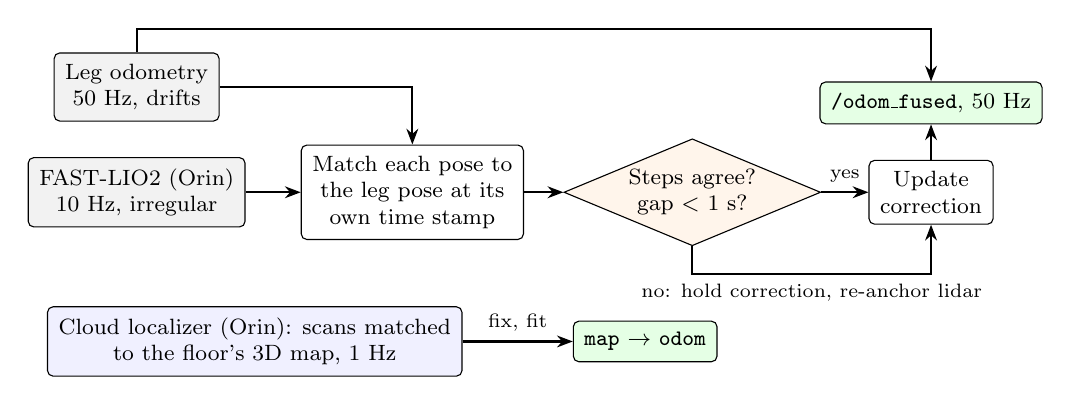
\begin{tikzpicture}[node distance=0.4cm and 0.6cm]
  \node[dev] (leg) {Leg odometry\\ 50 Hz, drifts};
  \node[dev, below=0.45cm of leg] (lio) {FAST-LIO2 (Orin)\\ 10 Hz, irregular};
  \node[box, font=\footnotesize, right=0.7cm of lio] (match) {Match each pose to\\ the leg pose at its\\ own time stamp};
  \node[dec, right=0.5cm of match] (gate) {Steps agree?\\ gap $<$ 1 s?};
  \node[box, font=\footnotesize, right=0.6cm of gate] (corr) {Update\\ correction};
  \node[box, font=\footnotesize, fill=green!10, above=0.45cm of corr] (fused) {\texttt{/odom\_fused}, 50 Hz};
  \draw[arr] (lio) -- (match);
  \draw[arr] (leg) -| (match.north);
  \draw[arr] (match) -- (gate);
  \draw[arr] (gate) -- node[lbl, above] {yes} (corr);
  \draw[arr] (gate.south) -- ++(0,-0.35) -| node[lbl, pos=0.25, below] {no: hold correction, re-anchor lidar} (corr.south);
  \draw[arr] (corr) -- (fused);
  \draw[arr] (leg.north) -- ++(0,0.3) -| (fused.north);
  \node[box, font=\footnotesize, fill=blue!6, below=1.0cm of lio, xshift=1.5cm] (cl) {Cloud localizer (Orin): scans matched\\ to the floor's 3D map, 1 Hz};
  \node[box, font=\footnotesize, fill=green!10, right=1.4cm of cl] (mo) {\texttt{map}~$\to$~\texttt{odom}};
  \draw[arr] (cl) -- node[lbl, above] {fix, fit} (mo);
\end{tikzpicture}
\caption{How the odometry and the map position were formed. The legs gave the rate, FAST-LIO2
removed their drift, and the cloud localizer placed the odometry frame on the map.}
\label{fig:odom}
\end{figure}

\section{Mapping and Localization}

A floor map was made from one walk: the operator started a recording in the panel, walked the robot with
the handheld and saved it. FAST-LIO2's point cloud became the floor's 3D map, and a 2D map was sliced from
it at wall height, with cells within 0.6~m of the walked path marked free so that doors passed through
stayed open. To place the robot, the operator tapped its position and heading on the map. The Orin then
matched FAST-LIO2's scans to the 3D map with ICP about once per second, refusing to place the robot
while FAST-LIO2's frame was more than 1.5$^\circ$ off level, and the fixes were smoothed into the \texttt{map} to
\texttt{odom} transform. One node published whether the robot was localized, and a navigation goal
refused to start, or stopped, without it.

\section{Navigation}

Navigation could run in two modes. In \emph{mapless} mode, everything ran on the perception computer in
the odometry frame, using the vendor's Nav2 configuration with RPP. In \emph{map mode}, used on campus,
planning and control ran on the Orin, as shown in Figure~\ref{fig:nav}.

\begin{figure}[htbp]
\centering
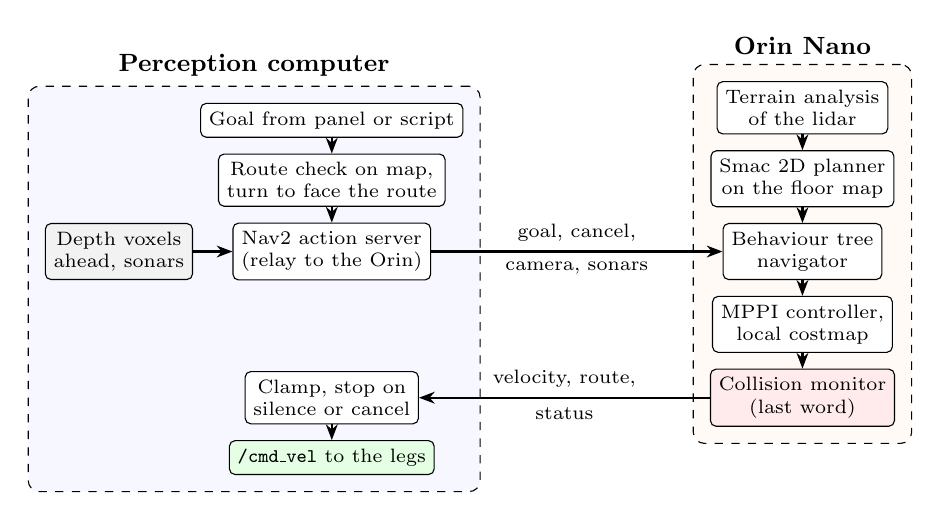
\begin{tikzpicture}[node distance=0.2cm and 0.45cm, b/.style={box, font=\scriptsize, inner sep=3pt}]
  \node[b] (goal) {Goal from panel or script};
  \node[b, below=of goal] (route) {Route check on map,\\ turn to face the route};
  \node[b, below=of route] (srv) {Nav2 action server\\ (relay to the Orin)};
  \node[b, fill=gray!10, left=0.5cm of srv] (sens) {Depth voxels\\ ahead, sonars};

  \node[b, right=3.7cm of srv] (bt) {Behaviour tree\\ navigator};
  \node[b, above=of bt] (smac) {Smac 2D planner\\ on the floor map};
  \node[b, above=of smac] (terr) {Terrain analysis\\ of the lidar};
  \node[b, below=of bt] (mppi) {MPPI controller,\\ local costmap};
  \node[b, fill=red!8, below=of mppi] (cm) {Collision monitor\\ (last word)};

  \node[b] (clamp) at (srv |- cm) {Clamp, stop on\\ silence or cancel};
  \node[b, fill=green!10, below=of clamp] (cmd) {\texttt{/cmd\_vel} to the legs};

  \begin{scope}[on background layer]
    \node[group, fill=blue!3, fit=(goal)(cmd)(sens), label={[font=\small\bfseries]above:Perception computer}] {};
    \node[group, fill=orange!4, fit=(terr)(cm), label={[font=\small\bfseries]above:Orin Nano}] {};
  \end{scope}

  \draw[arr] (goal) -- (route);
  \draw[arr] (route) -- (srv);
  \draw[arr] (sens) -- (srv);
  \draw[arr] (srv) -- node[lbl, above] {goal, cancel,} node[lbl, below] {camera, sonars} (bt);
  \draw[arr] (terr) -- (smac);
  \draw[arr] (smac) -- (bt);
  \draw[arr] (bt) -- (mppi);
  \draw[arr] (mppi) -- (cm);
  \draw[arr] (cm) -- node[lbl, above] {velocity, route,} node[lbl, below] {status} (clamp);
  \draw[arr] (clamp) -- (cmd);
\end{tikzpicture}
\caption{Map-mode navigation. The perception computer kept the map, the goal interface and the final
say over the legs; the Orin planned and controlled. The link between them was UDP.}
\label{fig:nav}
\end{figure}

The perception computer kept the map, its costmaps and a planner, used to draw routes and check that a
goal was reachable; if the route left more than 60$^\circ$ from the robot's heading, the robot first
turned to face it. A relay acting as Nav2's standard action server passed the goal to the Orin, where a
behaviour tree ran the Smac 2D planner~\cite{smac} and the MPPI controller. The local costmap combined
the lidar, through the terrain analysis of the Carnegie Mellon University (CMU) stack~\cite{cmu}, with
depth camera voxels for the blind spot in front of the robot. A collision monitor had the last word,
slowing or stopping the robot for anything close ahead, including glass seen only by the front sonar.
The perception computer clamped the returned commands to $-0.2$--0.5~m/s and $\pm$0.8~rad/s and
published them only during a goal. It stopped publishing after 0.3~s without the Orin, the Orin cancelled
its goal after one second without the perception computer, and no commands were sent without fresh
camera and sonar data.

\section{Operator Interface and Speech}

The robot was supervised through a password-protected web panel, reached over the VPN or the robot's own
Wi-Fi. It showed live status, both cameras, a 3D model of the robot with Nav2's path and the floor map, from
which the operator sent goals, recorded maps and drove the robot. The
joystick was a dead-man switch that halted the robot 0.3~s after the last stick message; a goal was
cancelled 10~s after the last page disconnected, long enough to ride out a Wi-Fi hand-over, and became an
emergency stop if Nav2 did not let go. These stops depend on the software and the network, so during
tests a person with the handheld stayed near the robot. Speech was synthesized by the Kokoro
model~\cite{kokoro} on the Orin's graphics processor and streamed sentence by sentence to the loudspeaker through a compressor and limiter.

\section{Testing and Results}

Table~\ref{tab:results} lists the measurements. Navigation ran on maps recorded by the robot, with
people moving around it and a person carrying the handheld.

\begin{table}[!t]
\centering\footnotesize
\caption{Measured results. Navigation times are from goal sent to goal reached.}
\label{tab:results}
\begin{tabular}{@{}p{0.22\linewidth}p{0.75\linewidth}@{}}
\toprule
Test & Result \\
\midrule
Odometry, walked loop & 10.4~m loop in 92~s: FAST-LIO2 ended 0.05~m from the start, leg odometry 0.21~m \\
Leg odometry scale & 1.712~m by odometry against 1.960~m by tape, corrected by a factor of 1.15 \\
Turns & $\pm$30$^\circ$ requests settled at 29.3--30.3$^\circ$ after compensating a 0.17~s coast \\
E-stop under Nav2 & 0.000~m travelled after \texttt{estop()} during an active goal \\
Through a lab door & out and back: 2 of 2 goals, 11.7~s and 11.3~s, no recoveries, median 0.48~m/s \\
MPPI against RPP & door route, both on the perception computer: about 10~s each way with MPPI, 14--15~s
  with RPP (0.16--0.18~m/s in the doorway) \\
Lab and hall & 7 of 7 goals reached \\
Lab to the arcade & over a bridge and back: 3 of 3 goals, outward leg 200~s with four glare stops, recoveries on the return \\
Speech & 0.4~s to synthesize a sentence, 0.6--0.7~s from Say to sound \\
Remote link & 6~ms VPN round trip to the robot over the campus Wi-Fi \\
\bottomrule
\end{tabular}
\end{table}

The main remaining fault was on the bridge: facing the low sun, glare on the glossy floor appeared to the
depth camera as small obstacles 0.5~m ahead, which stopped the robot several times until it replanned.
Localization could also not detect sliding along a featureless corridor, metal-grid fences gave false
depth readings, and FAST-LIO2 had to be restarted if it started while the robot was settling.

\section{Further Work}
\label{sec:further}

The parts of the project description not covered here are the plan for a master thesis: reinforcement
learning, for example Proximal Policy Optimization (PPO), for navigation or locomotion, trained in
simulation (Gazebo or Isaac Sim) on the robot model already used in RViz; the remaining sensors, a
millimetre-wave radar, a thermal camera, GPS and an environmental sensor, calibrated and time-synchronized
with the lidar and IMU; and the move from campus to industrial inspection, with stairs, uneven ground and
inspection missions. The current stack needs a hardware remote stop, so that no one has to stay near the robot, and a check
of the depth camera against the lidar for glare.

\section{Conclusion}

The research question asked how an off-the-shelf quadruped could navigate a building autonomously,
safely and under remote supervision. \emph{Autonomously}: once a floor had been mapped and the robot
placed on it, it planned and walked to goals by itself, reaching every goal in the tests, including the
route across the bridge. \emph{Safely}: the \texttt{Lite3} class ended every motion with a stop, the
emergency stop halted the robot within the test's resolution, and a collision monitor and timeouts
covered the rest, with the handheld as the only hardware stop. \emph{Under remote supervision}: one operator
followed and commanded the robot from the web panel over the campus network.

{\footnotesize\raggedright
\begin{thebibliography}{99}\setlength{\itemsep}{-1pt}\setlength{\parsep}{0pt}
\bibitem{deeprobotics} DEEP Robotics, ``Lite3 quadruped robot,'' \url{https://www.deeprobotics.us/products/lite-3/}, 2026.
\bibitem{ros2} S. Macenski, T. Foote, B. Gerkey, C. Lalancette and W. Woodall, ``Robot Operating
  System 2: Design, architecture, and uses in the wild,'' \emph{Science Robotics}, vol.~7, no.~66, 2022.
\bibitem{realsense} Intel, ``RealSense depth camera D435i,'' \url{https://www.intelrealsense.com}, 2026.
\bibitem{livox} Livox Technology, ``Mid-360 lidar,'' \url{https://www.livoxtech.com/mid-360}, 2026.
\bibitem{fastlio2} W. Xu, Y. Cai, D. He, J. Lin and F. Zhang, ``FAST-LIO2: Fast direct lidar-inertial
  odometry,'' \emph{IEEE Trans.\ Robotics}, vol.~38, no.~4, pp.~2053--2073, 2022.
\bibitem{icp} P. J. Besl and N. D. McKay, ``A method for registration of 3-D shapes,'' \emph{IEEE
  Trans.\ Pattern Analysis and Machine Intelligence}, vol.~14, no.~2, pp.~239--256, 1992.
\bibitem{nav2} S. Macenski, F. Martín, R. White and J. Ginés Clavero, ``The Marathon 2: A navigation
  system,'' in \emph{Proc.\ IEEE/RSJ IROS}, 2020.
\bibitem{smac} S. Macenski, M. Booker and J. Wallace, ``Open-source, cost-aware kinematically feasible
  planning for mobile and surface robotics,'' arXiv:2401.13078, 2024.
\bibitem{mppi} G. Williams et al., ``Information theoretic MPC for model-based reinforcement
  learning,'' in \emph{Proc.\ IEEE ICRA}, 2017.
\bibitem{cmu} J. Zhang et al., ``Autonomy stack for the Unitree Go2,'' CMU, \url{https://github.com/jizhang-cmu/autonomy_stack_go2}, 2026.
\bibitem{anymal} M. Hutter et al., ``ANYmal --- a highly mobile and dynamic quadrupedal robot,'' in
  \emph{Proc.\ IEEE/RSJ IROS}, 2016.
\bibitem{rpp} S. Macenski, S. Singh, F. Martín and J. Ginés, ``Regulated pure pursuit for robot path
  tracking,'' \emph{Autonomous Robots}, vol.~47, pp.~685--694, 2023.
\bibitem{robotloc} T. Moore and D. Stouch, ``A generalized extended Kalman filter implementation for
  the Robot Operating System,'' in \emph{Proc.\ Intelligent Autonomous Systems 13}, 2014.
\bibitem{kokoro} hexgrad, ``Kokoro-82M,'' \url{https://huggingface.co/hexgrad/Kokoro-82M}, 2025.
\end{thebibliography}
}

\end{document}
